\documentclass[letter,french]{report}
\usepackage[T1]{fontenc}
\usepackage[utf8]{inputenc} 
\usepackage{lmodern}
\usepackage{babel}
\usepackage[pdftex]{graphicx}
\usepackage[nointegrals]{wasysym}
\usepackage{amsmath,amssymb}


\begin{document}
	\title{Devoir 1 IFT 3913}
	\author{Ludovic André et Gevrai Jodoin-Tremblay}
	\date{Remis le 5 Octobre 2017}
	\maketitle
	
	
	\subsection*{Description du logiciel}
	Ce logiciel affiche une interface usager simple, très semblable
	à l'exemple d'interface usager de l'énoncé du travail pratique. Le bouton "Charger
	fichier" ouvre une fenêtre système permettant de sélectionner un fichier .ucd.
	Lorsqu'un fichier est choisi, il est \emph{parser} et ses éléments sont affichés dans
	les champs correspondants de l'interface. L'usager peut selectionner les
  différents éléments de l'interface pour avoir plus de détails sur ceux-ci.
	
	\subsection*{Lignes de compilation}
	Nous avons opté pour un \emph{makefile} histoire de rendre la compilation et l'exécution
	la plus facile possible sur les machines du DIRO. Un simple \emph{make} compile
	l'entièreté du logiciel et l'exécute. Pour voir les autres options, \emph{make help}
	explique les différentes commandes possibles.
	
	\section*{Conception}
	
	\subsection*{Interface Usager : Pattern MVC}
	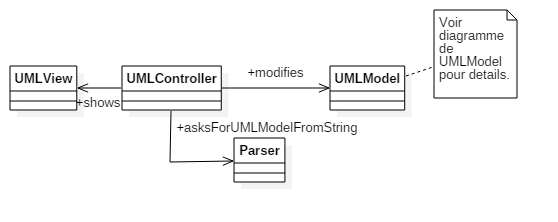
\includegraphics[scale=.7]{MVC_diagram.png}
  Après discussions au sein de notre équipe, nous avons opté pour le
  patron Modèle-Vue-Controlleur pour dirigé l'interaction entre l'interface
  usager et le modèle \emph{UML} reçu du parseur. Ce patron permet une
  séparation nette entre l'interface et les données en passant par le biais du
  controlleur qui dirige absolument tous. Ainsi, la classe \emph{UMLController}
  s'occupe de répondre aux évènements des éléments de \emph{UMLView}, de
  quérir et changer le \emph{UMLModel} courant.

	De cette manière, on s’assure que notre application à une forte cohésion et
  un faible couplage. Aussi, si jamais on veut créer une nouvelle vue ou
  modifier la vue existante, on peut facilement le faire sans avoir à changer
  la logique même du programme.
	
	\subsection*{Représentation des éléments UML}
	L'image suivante montre le diagramme de Classe de notre représentation des
  éléments \emph{UML}. Il est à noter que pour rendre le diagramme le plus
  lisible possible nous n'avons pas inclus les opérations des classes et n'avons
  garder que les attributs de bases.
	\newline 
	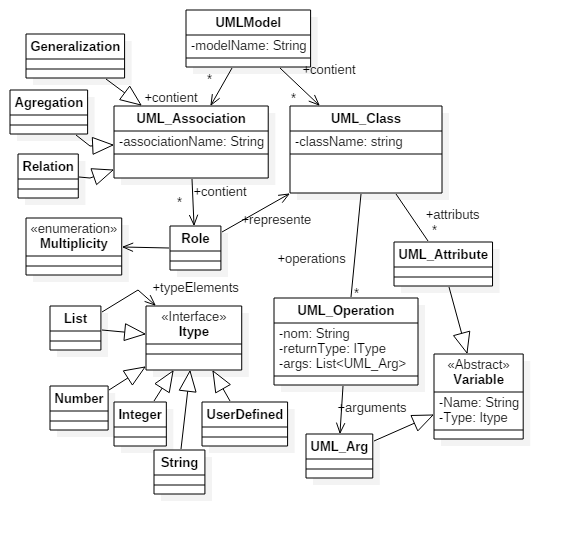
\includegraphics[scale=.7]{UML_diagram.png}

  La classe \emph{UMLModel} se trouve à la tête de la représentation et
  contient tous les éléments du fichier \emph{.ucd} d'entrée.

  Les différents types d'associations sont tous des sous-classes de
  \emph{UMLAssociation} et contiennent des \emph{Role}, contenant la
  \emph{UMLClass} impliqué ainsi qu'une \emph{Multiplicity} représentant le
  nombre d'éléments impliqués.

  Le modèle contient évidemment aussi des \emph{UMLClass} qui eux mêmes ont des
  \emph{Operation} et des \emph{Attributes}. Les opérations ont une liste
  d'\emph{Argument} qui est sous-classe de \emph{Variable}, tous comme les
  attributs des classes. Bien que, à toutes fins pratiques dans notre
  implémentation il n'y ai pas de différences entre ces deux sous-classes, nous
  étions d'avis que la différence logique entre un attribut et un argument
  demandait des classes distinctes.

  Finalement, \emph{IType} défini une interface pour les types \emph{UML} de
  base ainsi que les types définis par l'utilisateur, soit les \emph{UMLClass}
  pré-définis.
  
	\section*{Implantation}
	
	\subsection*{Parseur}
	Le parseur est inclus dans une seule classe statique, dont la seule méthode
	publique \emph{parse} prend une liste de \emph{String} correspondants aux lignes d'un
	fichier \emph{.ucd} et renvoie le \emph{UMLModel} correspondant. 
	
	Le \emph{parsing} est majoritairement effectué avec des expressions régulières,
	principalement parce que la grammaire \emph{BNF} donnée dans l'énoncé s'y
	prêtait particulièrement bien. Ainsi, on découpe le texte en de plus en plus
	petits tronçons et ont créer les objets du paquet \emph{uml} directement.
	
	\subsection*{MVC}
  La classe UMLView offre des méthodes permettant d'accrocher des
  \emph{Listeners} aux différents éléments de l'interface. \emph{UMLController} créer
  ces \emph{Listeners} et leurs associes des méthodes changeants l'état de
  l'interface et du UMLModel. Cette implémentation du patron MVC est très de
  base, mais démontre bien ces avantages, soit sa modularité et la forte
  cohésion des différentes parties du système. On pourrait très bien continuer
  le développement de ce logiciel en ajoutant d'autres vues et modèles, sans
  pour autant avoir à modifier ceux déjà existants car ils ne savent rien des
  autres composantes. Seul le controlleur est propre à cette application, ce qui
  est bien conforme au patron MVC.
	
	\section*{Problèmes rencontrés}
  Nous avons utilisé la librairie swing mais nous nous sommes confronté à des
  problèmes en tentant d'afficher correctement les éléments graphiques.
  Nous éprouvions des difficultés à afficher toute l'information dans les cases
  si les noms des attributs,méthodes,associations ou sous-classes étaient trop longs.

  Le parsing était éprouvant aussi, principalement parce qu'il était difficile
  de tester les méthodes à chacune des étapes, mais aussi car c'était notre
  première vrai expérience avec les \emph{REGEX}. Nous avions en fait commencer
  le parsing avec la librairie externe \emph{ANTLR} qui semblait efficace, mais
  suite aux commentaires de l'auxiliaire de cours ne le conseillant pas, nous
  avons choisi de développer notre propre implémentation du parseur.

	\section*{Développements futur}
	Il serait très utile de pouvoir modifier un modèle UML directement à partir de l'interface,
	et permettre l'exportation du modèle ainsi modifier vers un fichier /.ucd/.
	
	
\end{document}
